\newpage
\begin{Pro}
   Para los siguientes DFA obten el DFA mínimo:
\end{Pro}

\begin{enumerate}
    \item 
    \item 
    \begin{figure}[h]
        \centering
        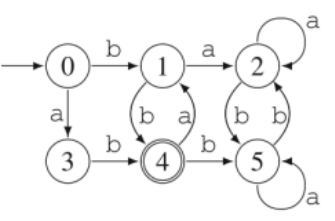
\includegraphics[width=0.5\textwidth]{images/ejercicio6b.png}
        \caption{Automata Finito Determinista, ejercicio 6 b}
    \end{figure}
    Separemos nuestros estados en dos grupos: los estados de aceptación y los que no lo son.
    \begin{itemize}
        \item Grupo 1 (aceptación): $\{q_4\}$
        \item Grupo 2 (no aceptación): $\{q_0, q_1, q_2, q_3, q_5\}$
    \end{itemize}

    Veamos como se comportarían los estados del Grupo 2 con las entradas posibles:
    \begin{table}[H]
    \centering
    \begin{tabular}{|c|c|c|}
    \hline
    \textbf{Estados} & \textbf{Transición con a} & \textbf{Transición con b } \\
    \hline
    $q_0$ & Grupo 1 & Grupo 1\\
    \hline
    $q_1$ & Grupo 1 & Grupo 2 \\
    \hline
    $q_2$  & Grupo 1 & Grupo 1 \\
    \hline
    $q_3$ & - & Grupo 2 \\
    \hline
    $q_5$ & Grupo 1 & Grupo 1 \\
    \hline
    \end{tabular}
    \caption{Tabla de ejemplo 6×3}
    \label{tab:ejemplo}
    \end{table}

\end{enumerate}

 Vamos a agrupar los estados que se comportan igual:
 \begin{itemize}
    \item Grupo A: $\{q_0, q_2, q_5\}$
    \item Grupo B: $\{q_1\}$
    \item Grupo C: $\{q_3\}$
 \end{itemize}
    Veamos como se comportarían los estados del Grupo A con las entradas posibles:      
    \begin{table}[H]
    \centering      
    \begin{tabular}{|c|c|c|}
    \hline
    \textbf{Estados} & \textbf{Transición con a} & \textbf{Transición con b } \\
    \hline
    $q_0$ & Grupo C & Grupo B\\     
    \hline
    $q_2$  & Grupo A & Grupo A \\       
    \hline
    $q_5$ & Grupo A & Grupo A \\    
    \hline
    \end{tabular}       
    \caption{Tabla de ejemplo 6×3}
    \label{tab:ejemplo}
    \end{table} 
    Ahora, agrupamos los estados que se comportan igual:
    \begin{itemize}     
        \item Grupo A1: $\{q_2, q_5\}$
        \item Grupo A2: $\{q_0\}$
        \item Grupo B: $\{q_1\}$
        \item Grupo C: $\{q_3\}$
    \end{itemize}
    Veamos como se comportarían los estados del Grupo A1 con las entradas posibles:      
    \begin{table}[H]        
    \centering      
    \begin{tabular}{|c|c|c|}        
    \hline
    \textbf{Estados} & \textbf{Transición con a} & \textbf{Transición con b } \\
    \hline
    $q_2$  & Grupo A1 & Grupo A1 \\ 
    \hline
    $q_5$ & Grupo A1 & Grupo A1 \\  
    \hline
    \end{tabular}       
    \caption{Tabla de ejemplo 6×3}
    \label{tab:ejemplo} 
    \end{table}
    Notemos que ambos estados se comportan igual, por lo que no es posible seguir dividiendo los grupos. Por lo tanto, los grupos finales son:
    \begin{itemize} 
        \item Grupo A1: $\{q_2, q_5\}$
        \item Grupo A2: $\{q_0\}$
        \item Grupo B: $\{q_1\}$
        \item Grupo C: $\{q_3\}$
        \item Grupo D (aceptación): $\{q_4\}$   
    \end{itemize}
    Ahora, construimos el DFA mínimo usando estos grupos como estados:
    \begin{figure}[h]
        \centering
        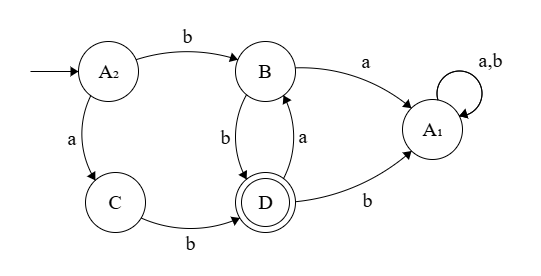
\includegraphics[width=0.5\textwidth]{images/6bresuelto.png}
        \caption{Automata Finito Determinista Minimo, ejercicio 6 b}
    \end{figure}
